% MorphGuard report: text and figures for §3.1, §3.2 and §5.2.
% Put this file's folder on the graphics path, e.g. \graphicspath{{docs/report/}}.
% The figures are vector PDFs (Fig. 1, 2) and a 300-dpi raster (Fig. 3); PNG copies sit beside them.

\section{Software Architecture \& System Design}

\subsection{High-Level System Architecture}

MorphGuard is a layered client--server system: a single-page web application talks to a REST API over HTTPS. The backend is a modular monolith. One Flask application, split into blueprints, serves every request. The long-running work runs as separate processes: Kafka stream processing, and batch training and evaluation jobs. Figure~\ref{fig:architecture} shows the five tiers.

\begin{itemize}
  \item \textbf{Client.} A React~18 single-page application built with Vite, with one page per sidebar item (Dashboard, Log Sources, Detection Results, Analytics, Smart Storage, Live Stream, Model Management and Settings). A shared REST client (\texttt{api.js}) attaches the user's JSON Web Token as a \texttt{Bearer} header. It also adds the selected log source (\texttt{?source=hdfs|openstack|apache|cloudtrail|django}) to every call. The client holds no business logic; every number on screen comes from the API.
  \item \textbf{Edge.} On the Google Cloud VM, nginx terminates HTTPS (Let's Encrypt), serves the built static files and reverse-proxies \texttt{/api} to gunicorn. systemd supervises the API service and one stream-processor service per log source.
  \item \textbf{API.} A Flask application on gunicorn with eight blueprints: authentication, account, pipeline (dashboard, detections, analytics, models, retraining), sources (uploads, connectors), storage, early warning, stream and feedback. Two cross-cutting pieces run on every request. \texttt{token\_required} validates the HS256 JWT. \texttt{source\_context} resolves the requested log source to its own models, vocabulary and reports, and returns 404 for a source that has not been built yet.
  \item \textbf{Services.} Domain modules called in-process by the API and by batch jobs:
  \begin{itemize}
    \item per-source parsers;
    \item feature engineering: cleaning, eight features per block, and a stable category vocabulary that every model is stamped with;
    \item Isolation Forest detection;
    \item genetic-algorithm optimisation with promote-if-better model evolution;
    \item Smart Storage tiering;
    \item early warning from a block's first $k$ events.
  \end{itemize}
  The streaming processes (producer, syslog receiver and stream processor) reuse the same feature code and models, so a live verdict matches the batch verdict.
  \item \textbf{Persistence.} Data is split by kind:
  \begin{itemize}
    \item MongoDB Atlas holds operational data: accounts, uploads, analyst feedback, and stream status and alerts.
    \item A version-controlled file store under \texttt{data/} holds the machine-learning artefacts: models, the model registry, evaluation reports and storage policies.
    \item Kafka (KRaft, one broker) carries the event stream.
    \item Raw datasets are downloaded on demand. HDFS, OpenStack, Apache and Django come from a public Hugging Face dataset; CloudTrail comes from the original flAWS archive, with each file's SHA-256 checksum checked.
  \end{itemize}
\end{itemize}

\textbf{Interaction.} A page request goes from the browser to nginx and then to gunicorn. There, the JWT check and source resolution run before a blueprint calls the service modules. Reads come from cached model and report files. Writes go to MongoDB. Slow work does not block a request:
\begin{itemize}
  \item an uploaded log is stored, recorded as \texttt{processing} and scored on a background thread, and the page polls its status;
  \item a retrain cycle runs as a background job, whose candidate model replaces the live one only if its F1 score is strictly higher.
\end{itemize}
In the streaming path, the producer or syslog receiver publishes lines to \texttt{logs.raw.<source>}. The stream processor groups them into blocks, scores them with the live model, and publishes alerts and storage decisions to Kafka. It also writes the run's status and alerts to MongoDB, which the Live Stream page polls every two seconds. Every component that scores data (API, uploads and stream) reads the live model through the same pointer, \texttt{current\_version.json}, so a promotion or rollback takes effect everywhere at once.

\begin{figure}[htbp]
  \centering
  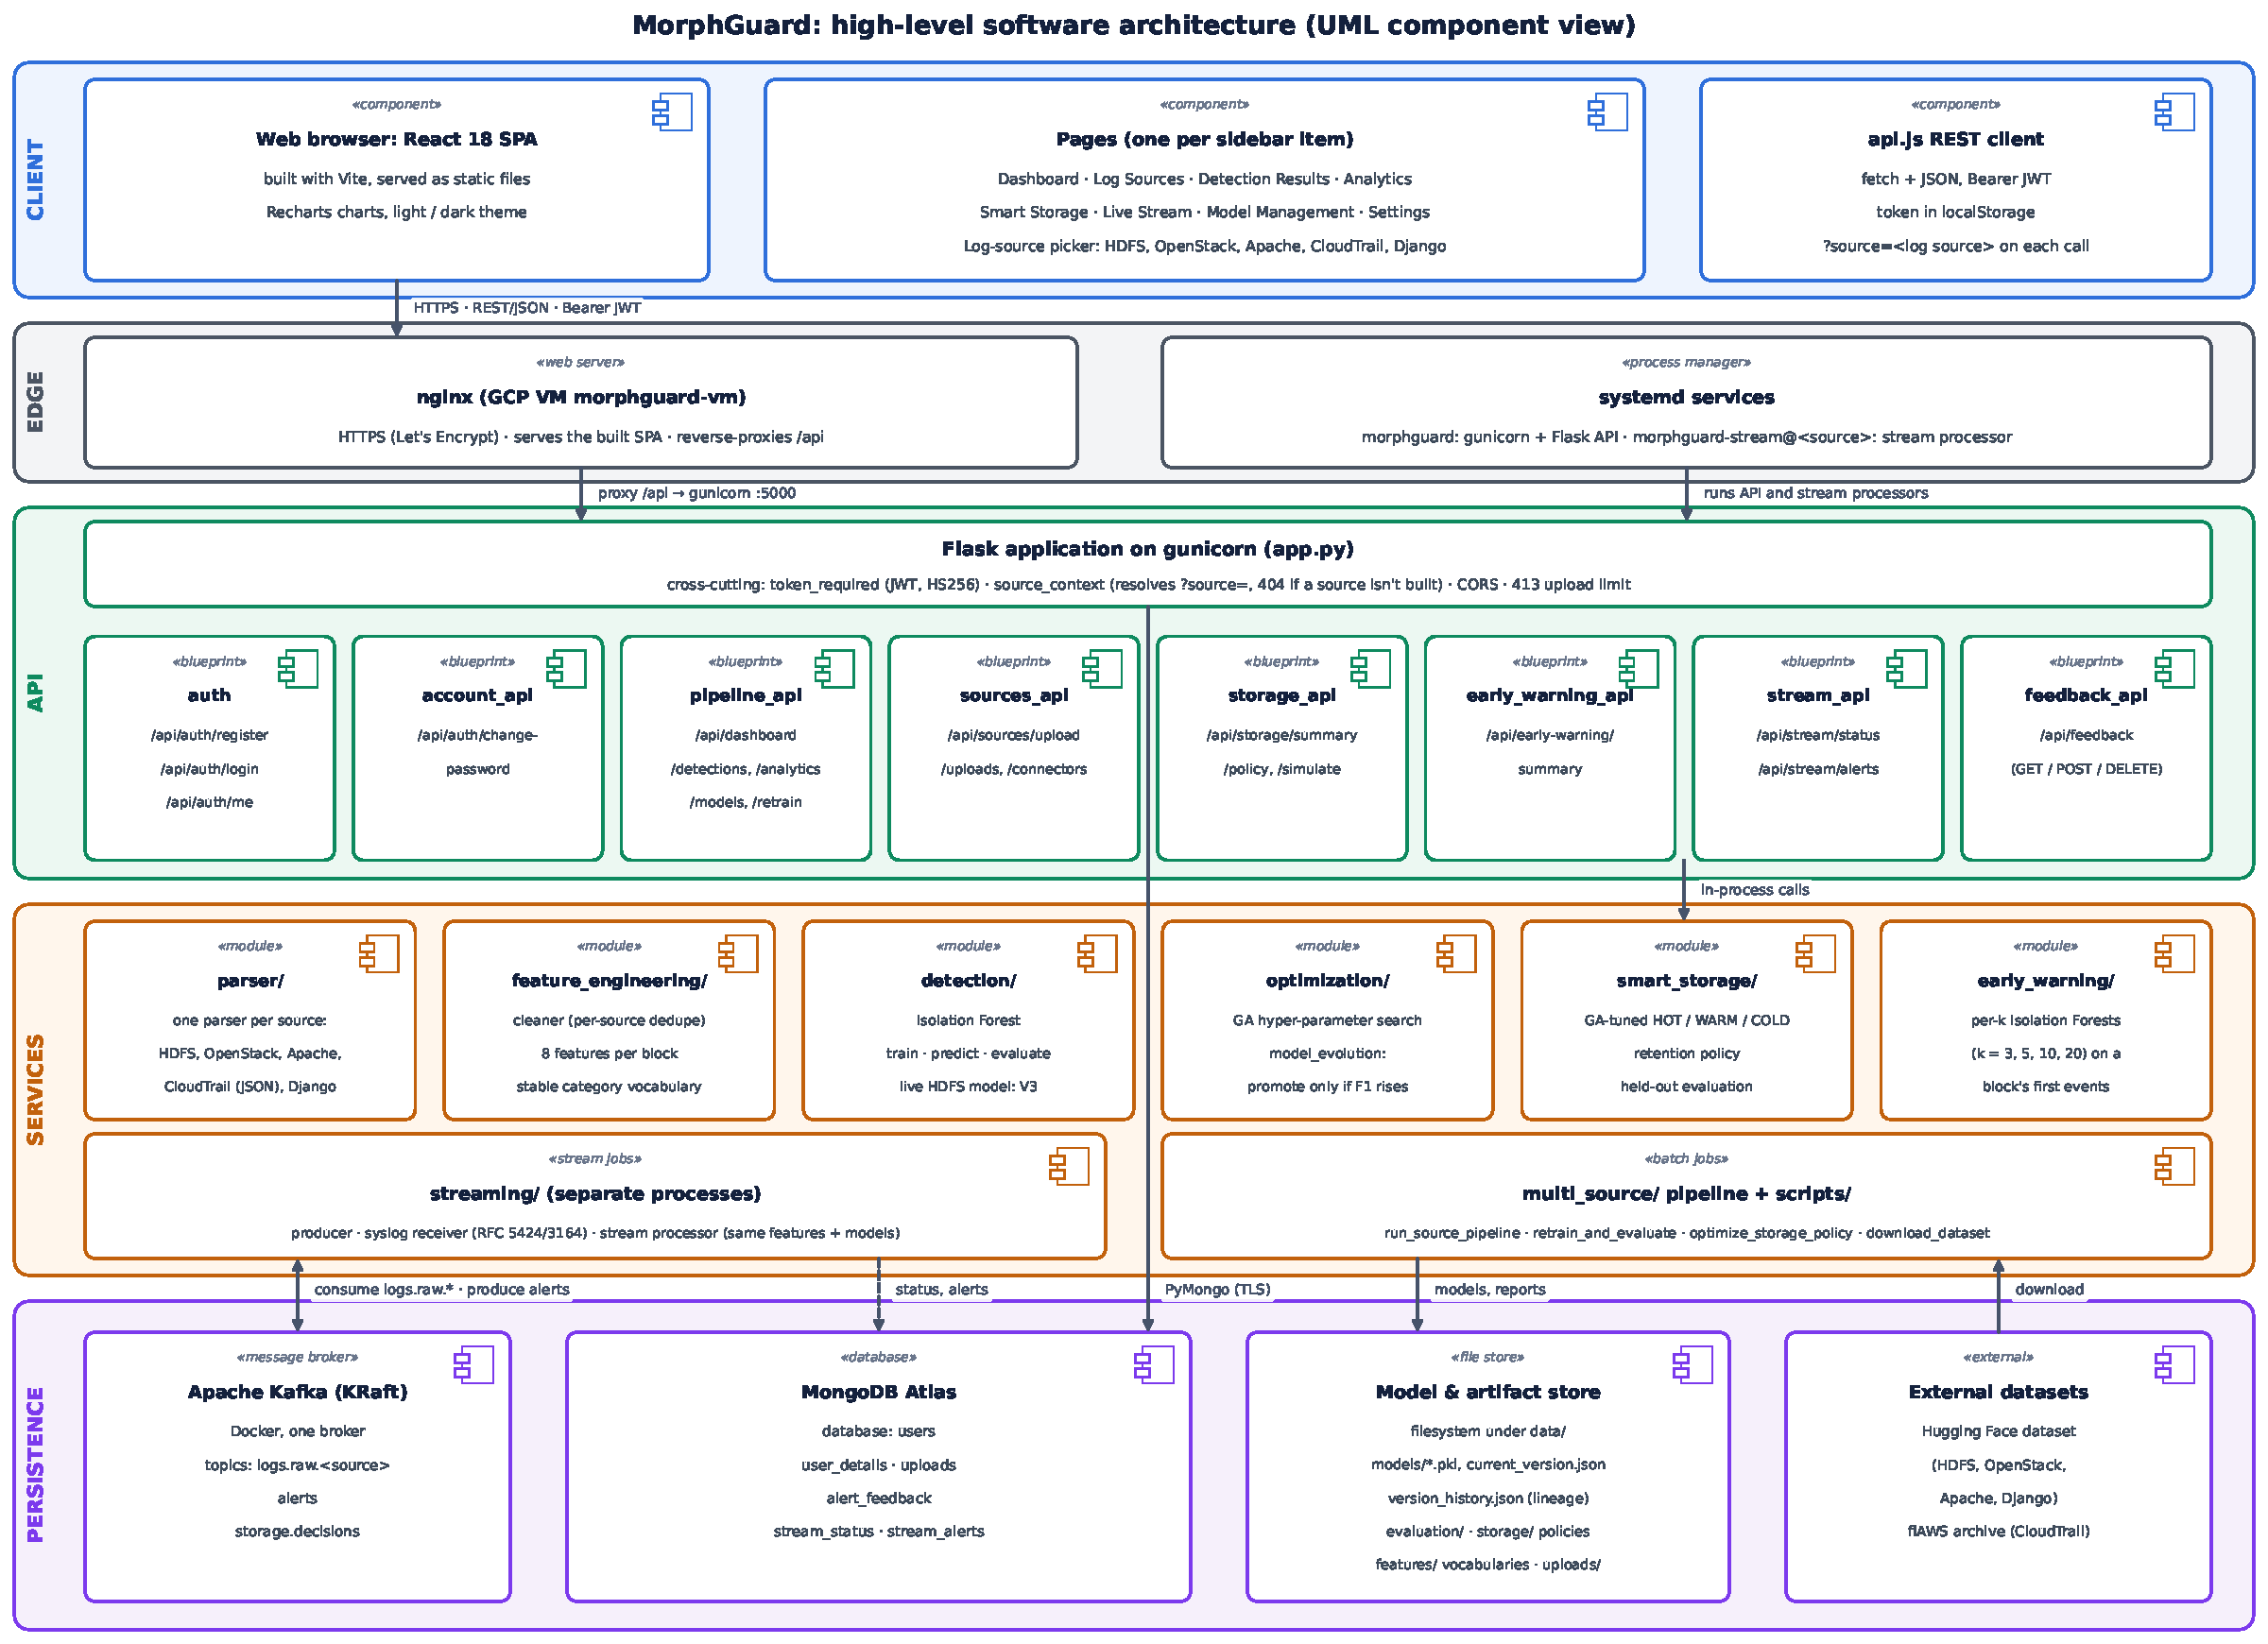
\includegraphics[width=\textwidth]{fig1_software_architecture.pdf}
  \caption{High-Level Software System Architecture}
  \label{fig:architecture}
\end{figure}

\subsection{Database Schema \& Data Modeling}

Operational data lives in a MongoDB Atlas database (\texttt{users}) with five collections, shown in Figure~\ref{fig:schema}. The model is document-oriented. Each document is self-contained. Nested objects hold related values, for example a stream run's alert and storage counters. Collections refer to each other through logical keys rather than joins.

\begin{itemize}
  \item \textbf{\texttt{user\_details}}: one document per account, holding email, display name, bcrypt password hash and timestamps. The email is the user's identity across the system.
  \item \textbf{\texttt{uploads}}: one document per uploaded log file. It records the file, its log source, a processing status (\texttt{processing}, \texttt{processed} or \texttt{failed}), the detection summary (blocks analysed, anomalies, anomaly rate), the model version that scored it, and provenance of the vocabulary and model used. It refers to its owner through \texttt{uploaded\_by}, the uploader's email.
  \item \textbf{\texttt{alert\_feedback}}: an analyst's verdict (\texttt{anomaly} or \texttt{normal}) on one block of one source, with a note, the analyst's email and a timestamp. The next retrain for that source uses these verdicts to override its training labels.
  \item \textbf{\texttt{stream\_status}}: one document per stream run, keyed by the run id and rewritten as the run progresses. It holds throughput, blocks in flight, alert and storage counters, the log-time watermark and the deployed model version.
  \item \textbf{\texttt{stream\_alerts}}: one document per alert (early warning or block anomaly), with its score, threshold, events seen and lead time. It refers to its run through \texttt{run\_id}.
\end{itemize}

\textbf{Relationships and cardinalities.} One user has zero or more uploads and zero or more feedback verdicts, both linked by email. One stream run has zero or more alerts, linked by \texttt{run\_id}. Each feedback verdict refers to one block in that source's labelled dataset. Uploads and stream runs record the model version that scored them, which refers to an entry in the file-based model registry. MongoDB does not enforce these references; the API maintains them.

\textbf{Constraints.}
\begin{itemize}
  \item \textbf{Unique email.} \texttt{user\_details.email} has a unique index, so sign-up rejects a duplicate account (HTTP 409).
  \item \textbf{One verdict per block.} Feedback is written as an upsert on \texttt{(source, block\_id)}, so each block of a source has exactly one verdict and the latest one wins.
  \item \textbf{Idempotent alerts.} An alert's \texttt{\_id} is \texttt{run\_id:type:block\_id}, so replaying the same events never creates a duplicate alert.
  \item \textbf{Validated values.} The API checks enumerated values (log sources, verdicts, statuses), password length, note length and upload size before writing.
  \item \textbf{No stored passwords.} Passwords are only ever stored as bcrypt hashes.
\end{itemize}

\textbf{Indexing strategy.} Indexes follow the queries the dashboard runs:
\begin{itemize}
  \item a unique index on \texttt{user\_details.email}, used for sign-in and the duplicate check;
  \item \texttt{stream\_status.updated\_at} descending, to fetch the latest run;
  \item a compound index on \texttt{stream\_alerts (run\_id, detected\_at desc)}, to page a run's alerts newest first.
\end{itemize}
\texttt{uploads} (looked up by owner, newest first) and \texttt{alert\_feedback} (looked up by source) are small enough to be scanned. Adding \texttt{(uploaded\_by, uploaded\_at)} and a unique \texttt{(source, block\_id)} index is the next step if they grow.

\textbf{File-based model registry.} Model artefacts are deliberately not stored in MongoDB: they are large binary files that must be versioned with the code. For each log source:
\begin{itemize}
  \item \texttt{current\_version.json} points to the live model, with its file, metrics and promotion time;
  \item \texttt{version\_history.json} is an append-only lineage of every promotion, rejection, refit, rollback and manual re-promotion, with the reason for each where one was given (the 9 Sep rollback's reason was not recorded);
  \item every model is stamped with the category vocabulary it was trained on, and scoring refuses to run if that vocabulary has changed.
\end{itemize}

\begin{figure}[htbp]
  \centering
  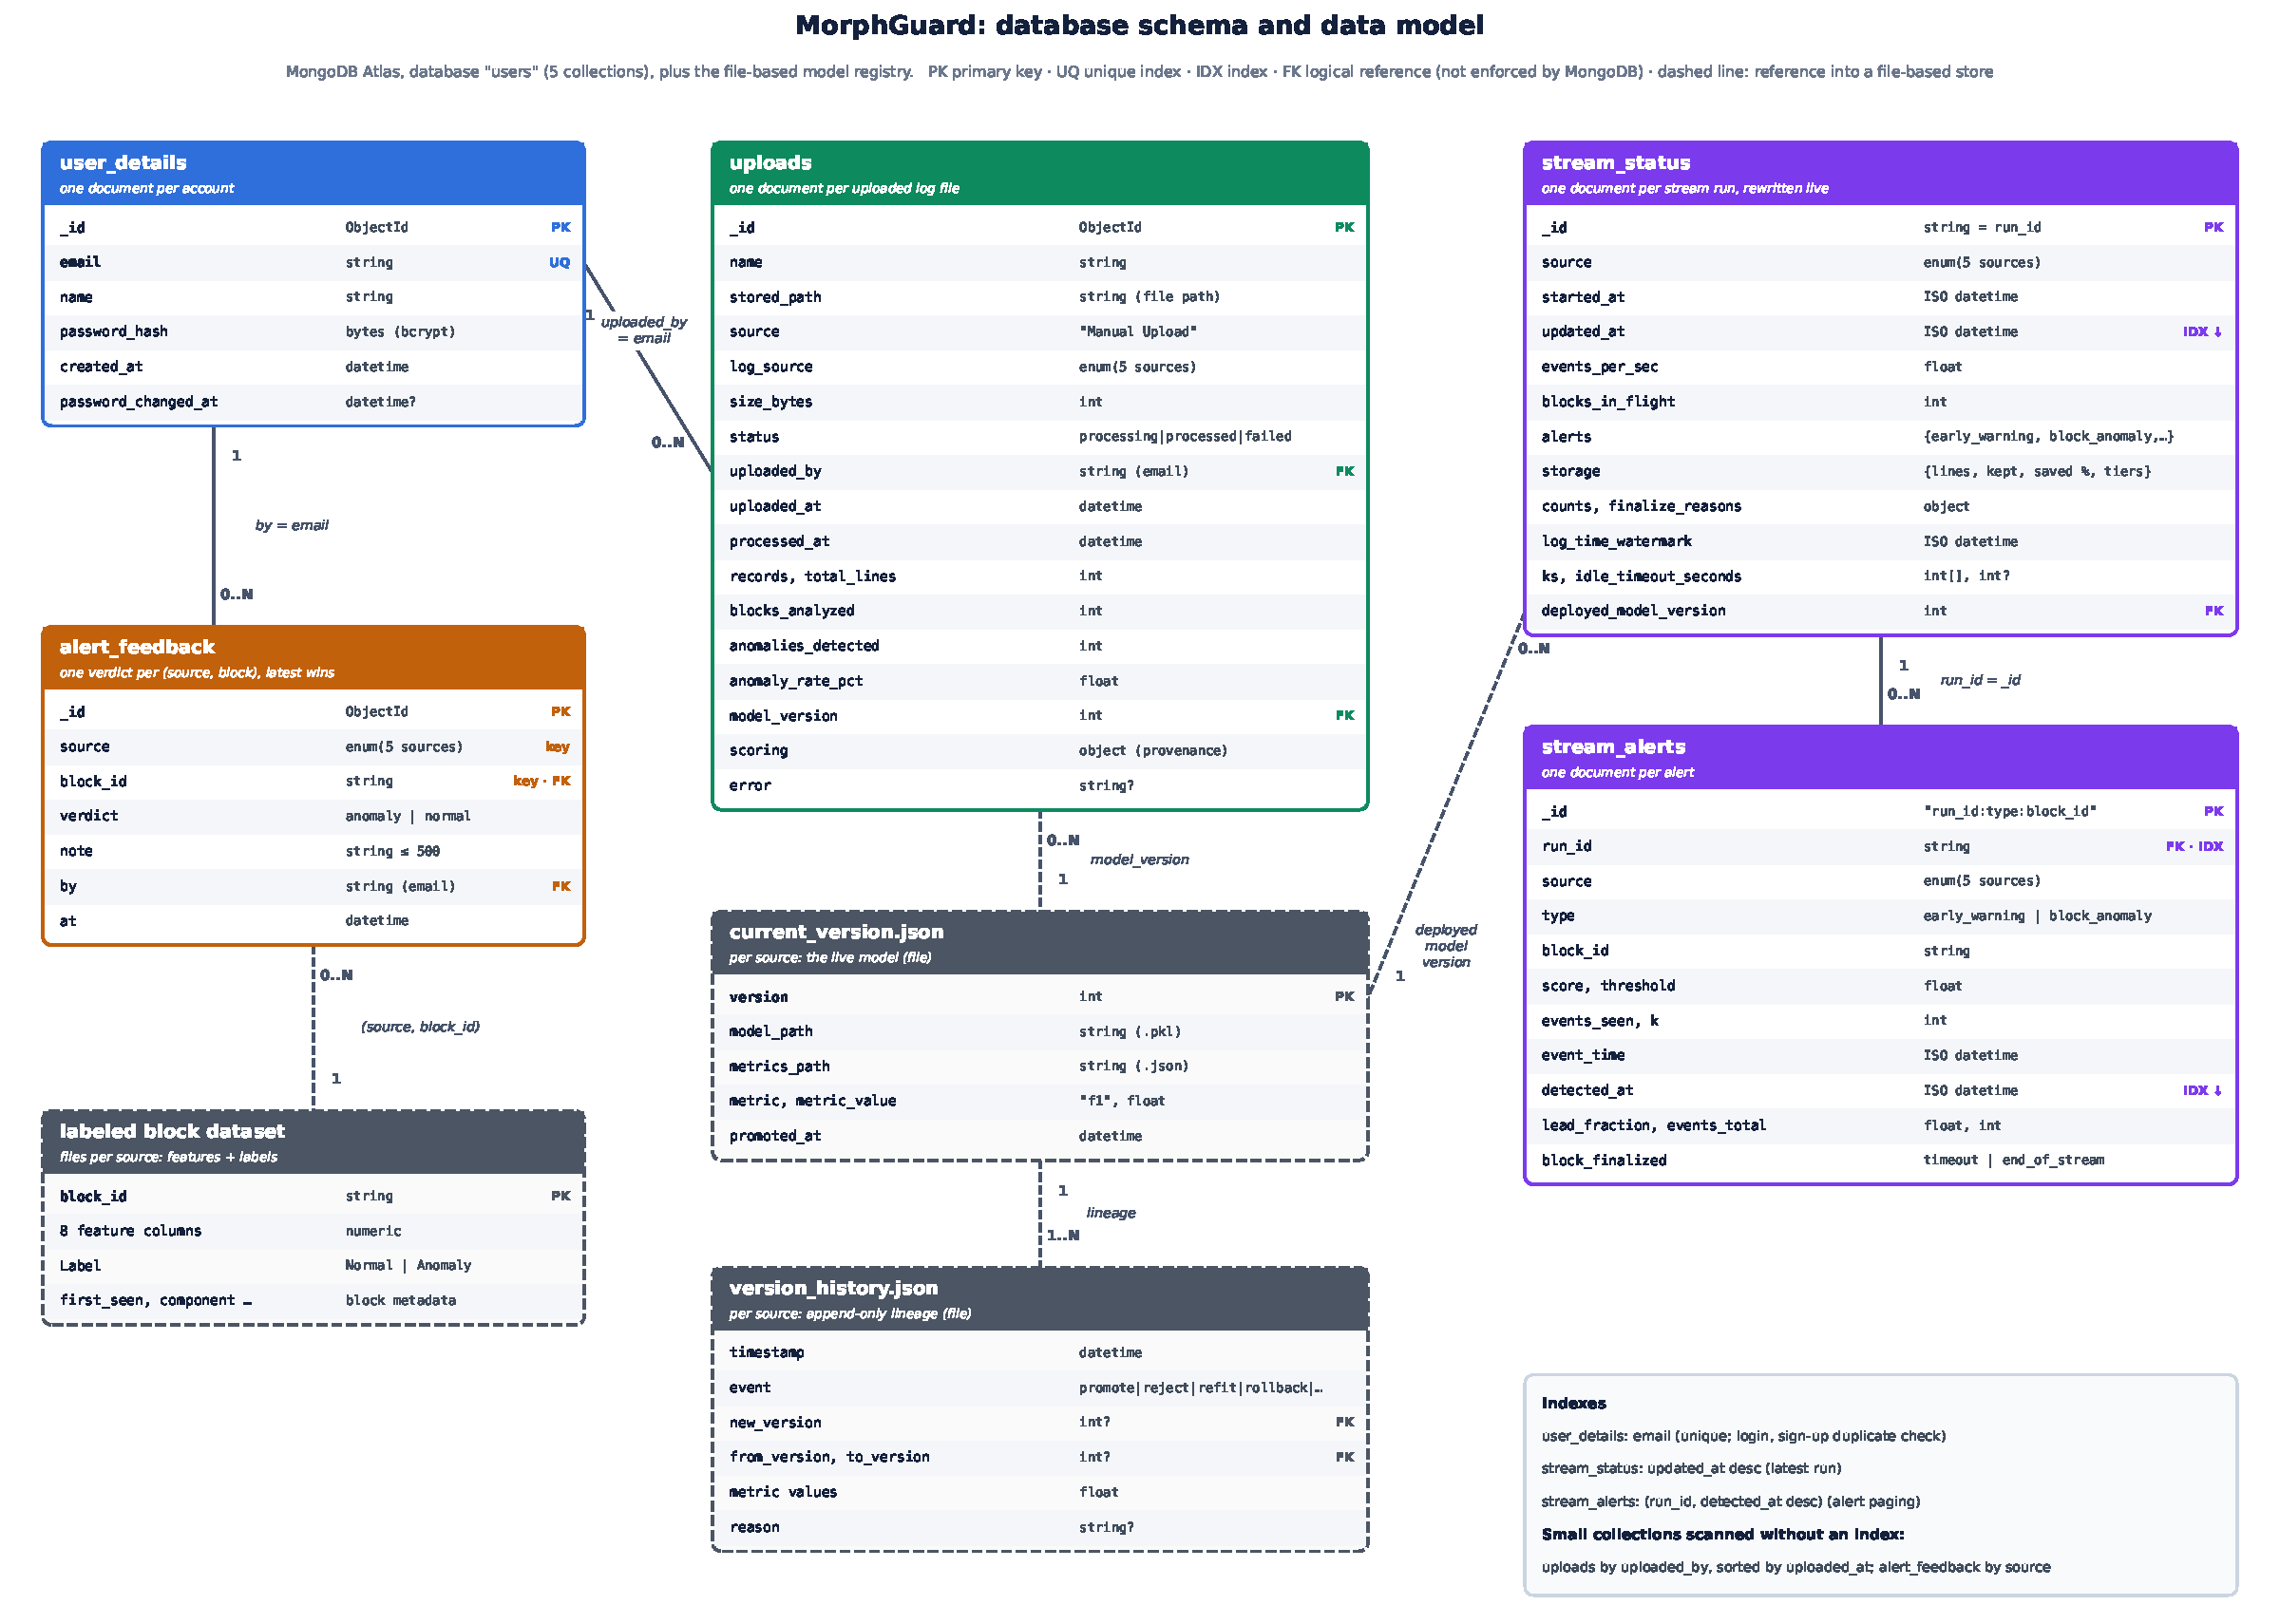
\includegraphics[width=\textwidth]{fig2_database_schema.pdf}
  \caption{Database Schema and Data Model Design}
  \label{fig:schema}
\end{figure}

% ---------------------------------------------------------------- §5.2
\subsection{System Demonstration \& Execution Views}

Figure~\ref{fig:demo} shows the running system:
\begin{itemize}
  \item \textbf{Panels (a)--(f): the application.} The dashboard on the full HDFS dataset with model V3 live; detection results with severity filtering and analyst verdicts; model management with held-out evaluation, the Autoencoder comparison and the model lineage; Smart Storage with its held-out results and policy simulator; a Live Stream run replayed through Kafka; and the log-source connectors.
  \item \textbf{Panel (g): the REST API.} Requests without a token are rejected (401). Then the API returns the dashboard figures, reports the model state, re-runs the storage policy, and returns clear errors for a source that has not been built (404) and an unknown source (400).
  \item \textbf{Panel (h): test verification.} The 204 automated tests pass, and continuous integration is green on both repositories.
\end{itemize}

\begin{figure}[htbp]
  \centering
  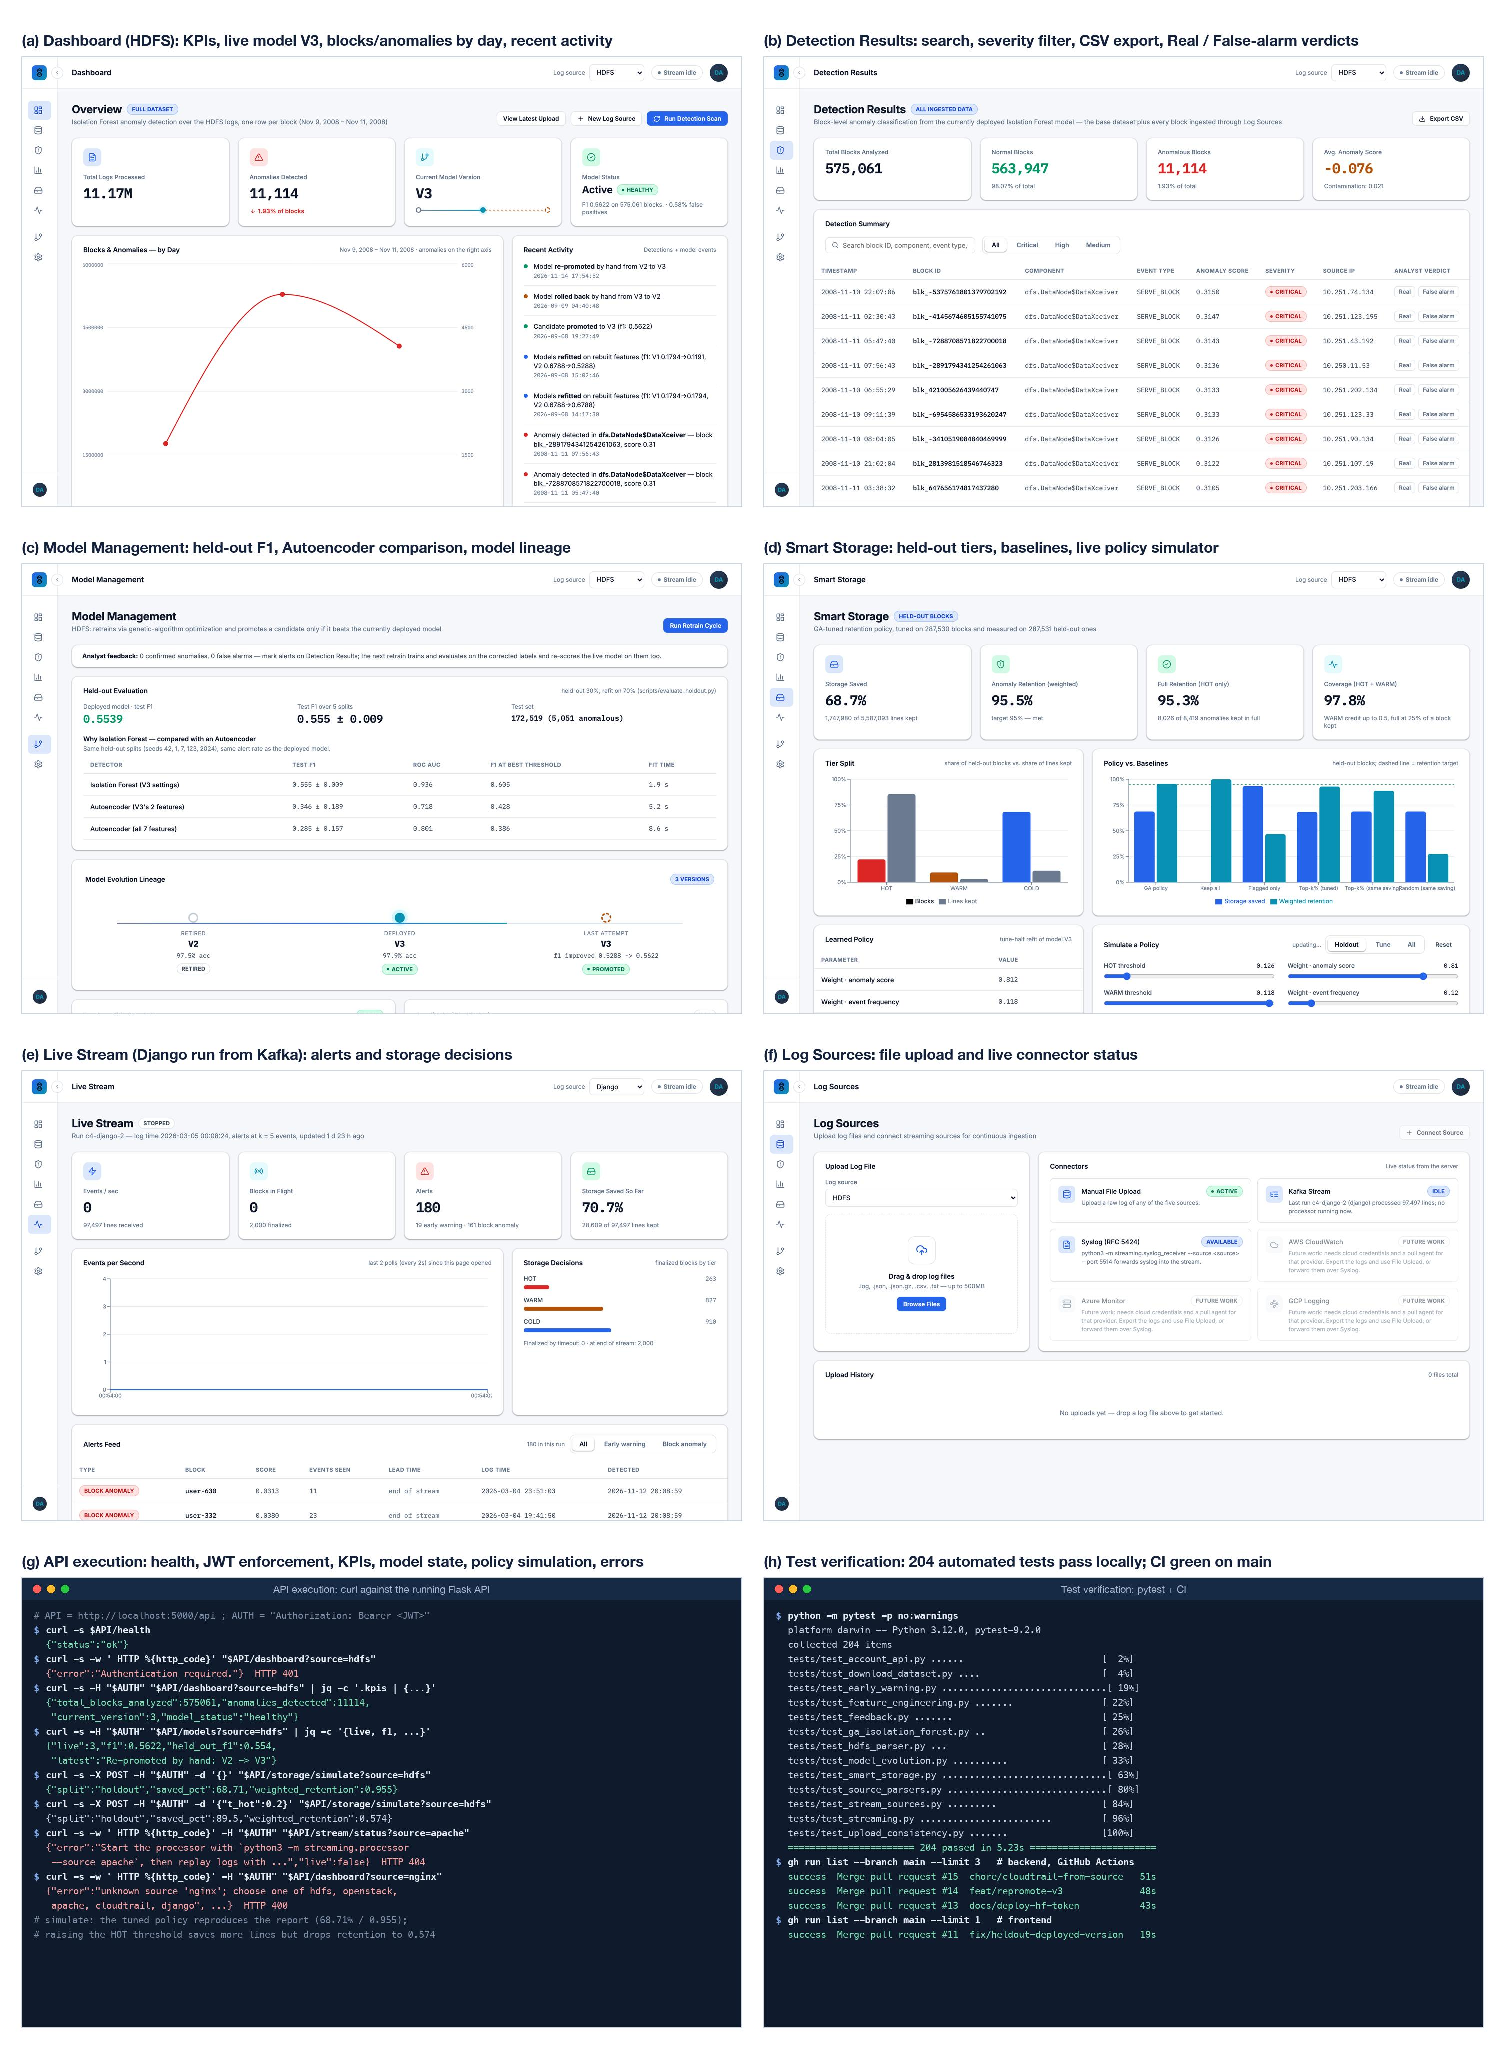
\includegraphics[width=\textwidth]{fig3_system_demonstration.pdf}
  \caption{Integrated Software System Demonstration and Test Execution Outputs}
  \label{fig:demo}
\end{figure}
